\chapter{Statistics Tool Box}
\label{chap:stat}

The data we collect is stochastic: quantum mechanics is not deterministic, the particle content result of an interaction follows probabilistic laws. Furthermore, experimental effects need to be taken into account. Therefore, a proper statistical treatment is essential to extract quantitative statements from the observed data. This chapter does not aim at being an exhaustive reference for statistics, but it describes the main statistical procedures that are used to obtain the results described in Chapter \ref{chap:strong_prod} and Chapter \ref{chap:ewk_prod}. After a brief introduction to statistical inference in Section \ref{sec:stat:intro}, the two main topics discussed are parameter estimation (Section \ref{sec:stat:pe}), that has the aim to determine the value of the input parameters that allows to best describe data, and hypothesis testing (Section \ref{sec:stat:ht}), that checks the plausibility of models against the observed data. 
%%%%%%%%%%%%%%%%%%%%%%%%%%%%%%%%%%%%%%%
\section{Statistical Inference}
\label{sec:stat:intro}

Statistical inference uses a data sample to make probabilistic statements on the population from which the sample is extracted. The generalization from the properties of the sample to the properties of the entire population comes with a certain degree of uncertainty, that can also be accesses through statistical methods.

There are two main approaches to statistical inference: Bayesian and frequentist.

\paragraph{Frequentist}

Probability is defined as the fraction of favorable outcomes of a repeatable experiment when the number of repetitions tends to infinity 
\begin{equation}
P(\mathrm{A}) = \lim_{N_{\mathrm{tot}} \rightarrow \infty} \frac{N_\mathrm{A}}{N_{\mathrm{tot}}}
\end{equation}

In the frequentist approach, there is no probability for hypothesis or true values of the parameters. A theory is either true or false, and given a theory only the data has a certain probability or probability density function (\pdf).

\paragraph{Bayesian}

In the Bayesian approach, probability is a more subjective notion, that incorporates the degree of belief in the from of priors. In this case it is meaningful to speak about \pdf not only for the observed data, but also for theories and parameters. Performing an experiment will modify the probability of a theory according to the Bayes formula:
\begin{equation}
P(\mathrm{theory} | \mathrm{data}) = \frac{ P(\mathrm{data}|\mathrm{theory}) \times P(\mathrm{theory})}{P(\mathrm{data})},
\end{equation}

\noindent where $P(\mathrm{data}|\mathrm{theory})$ is the probability of the data given the theory under examination, $P(\mathrm{theory})$ is the theory prior, $P(\mathrm{data})$ is a normalization constant that expresses the probability of observing these data whether the theory is true or false, and $P(\mathrm{theory} | \mathrm{data})$ is the final posterior probability of the theory.

In this chapter we discuss only about frequentist statistics, as only frequentist methods are applied to obtain the results presented in chapters \ref{chap:strong_prod} and chapter \ref{chap:ewk_prod}. 

As mentioned above, an hypothesis is statement based on which one can access the probability of the data. An hypothesis can be simple, when the data \pdf can be fully determined by stating if the hypothesis is true or false, or complex, when it depends on a number of parameters that in the following will be generally denoted with $\theta$. 

Given a certain hypothesis $H$, the probability of observing the data $x$ is $P(x|H)$. This probability can be considered also as a function of the hypothesis, for fixed data, and in this case it is assigned the name of \textit{likelihood} ($L$). In the case of a composite hypothesis, the value of the likelihood depends on the value of the parameters necessary to specify the hypothesis, and it takes the name of \textit{likelihood function}: $L(\theta)=P(x|\theta)$.

\section{Parameter Estimation}
\label{sec:stat:pe}

Parameter estimation, also know as \textit{fitting}, is the technique that allows to derive the best values of some parameters from data.
This sections describes parameter estimation and in particular the method based on the maximum likelihood.

\subsection{Estimators}

Consider a set of independent observations $\vec{x}=\{x_1, x_2, ..., x_\mathrm{N}\}$, distributed accordingly to a $\pdf$ $f(x|\vec{\theta})$, where $\vec{\theta}=\{\theta_1, \theta_2, ..., \theta_\mathrm{M}\}$ are the M true parameters that specify the underlying theory. 
A \textit{statistic} is any function of the measured data $\vec{x}$, and \textit{estimator} $\hat{\vec{\theta}}$ is a statistic introduced to provide an estimate of $\vec{\theta}$.

The characteristics used to evaluate the performance of an estimator are:


\paragraph{Consistency}
The asymptotic limit for large number of observations of the estimator is the true value of the parameter 
\begin{equation}
\label{eq:stat:consistency}
\lim_{N \rightarrow \infty} \hat{\vec{\theta}} = \vec{\theta}
\end{equation}


\paragraph{Bias}
The bias is the difference between the expectation value of the estimator ($E[\hat{\vec{\theta}}]$) and the true value
\begin{equation}
\label{eq:stat:bias}
b = E[\hat{\vec{\theta}}] - \theta
\end{equation}
Once the bias of a specific estimator is known, it is possible to build and unbiased one by defining 
\begin{equation}
\hat{\vec{\theta}}_{\mathrm{unbiased}} = \hat{\vec{\theta}} - b
\end{equation}


\paragraph{Efficiency}
The efficiency of an estimator is high when its variance ($V[\hat{\vec{\theta}}]$) is small. $V[\hat{\vec{\theta}}]$ has a lower bound, that is given by the Cramer-Rao inequality \cite{Cramer1946}\cite{Rao1992}.

%, stating that the variance is larger than the inverse of the information matrix $I[\theta]$
%\begin{equation}
%V[\hat{\vec{\theta}}] \geq I[\vec{\theta}]^{-1}
%\end{equation}

\paragraph{Robustness}
An estimator is robust if it is not sensitive to small changes in the assumptions in the \pdf


\subsection{The Maximum Likelihood Estimator}
\label{sec:stat:MLE}

The maximum likelihood estimate (MLE) of the parameters $\theta_i$, first introduced by Fisher \cite{fisher1911absolute}\cite{aldrich1997}, is obtained by choosing the set of parameters that yields the global maximum of the likelihood function. At an intuitive level this corresponds to the choice for which the observed data $\vec{x}$ are more probable. 

The MLE is widely used because of the favorable properties that it reaches in the asymptotic limit of infinite number of events N:
\begin{itemize}
\item Consistent, which means that it satisfies Eq. \ref{eq:stat:consistency}
\item Unbiased, so the bias, defined in Eq. \ref{eq:stat:bias}, tends to zero
\item Efficient, as it reaches the minimum bound for the variance 
\item It follows a Gaussian distribution
\end{itemize}
With a finite number of events, the estimator is biased and the bias is proportional to $\frac{1}{N}$. Also, the MLE is invariant under a functional transformation, which means that if $\hat{\theta}$ is the MLE for the parameter $\theta$, $g(\hat{\theta})$ is the MLE for the reparametrization $g(\theta)$ (and maintains therefore all the properties described above). This is not necessarily true for other estimators.

Practically, most of the times instead of maximizing the likelihood function is more convenient to minimize $-\logl$. This has the advantage to move from a maximization to a minimization because of the minus sign, but also to transform all the products into sums, which makes the minimization easier. As long as the likelihood is a monotonous function, its maxims are the same as the ones of the $\logl$.

There are two types of maximum likelihood fits that can be performed:
\begin{itemize}
\item \textit{Unbinned} fits, where each event enters in the likelihood separately. This method is the optimal one from the statistics point of view, but it results to be computationally expensive
\item \textit{Binned} fits, where the events are grouped in bins of a histogram, and the quantity entering in the likelihood is the number of events in each bin
\end{itemize}

In this chapter the focus will be on the second type of fit.

\subsubsection*{Variance of the Maximum Likelihood Estimator}

Given a data sample, to the estimate of a parameter is associated an uncertainty. If we would repeat the same parameter estimate on a different data sample, we would obtain a different values of the best estimate. If we repeat N times the same estimate on independent data samples, the best estimates will have a distribution that tends to a Gaussian for large N. There are two main methods to access the variance (and therefore the standard deviation) of this distribution.

\paragraph{Monte Carlo Method} Once the parameter is estimated from the experimental results, the experiment can be simulated N times with Monte Carlo simulations. For each simulation the best value of the parameter can be estimated with the maximum likelihood method, and from the distribution of these values it is possible to compute the variance.


\paragraph{Graphical Method} With the increase of the size of the data sample, the likelihood function tends to a Gaussian, and the $\logl$ tends to a parabola.  

\subsection{Binned Likelihood with Systematic Uncertainties}

If we consider the representation of the observed data given by the binned distribution of a certain variable, the expected number of events in each bin of the distribution is given by:

\begin{equation}
\label{eq:stat:exp}
E[n_i] = b_i + \mu s_i  \ ,
\end{equation}

\noindent where $b_i$ is the expected number of background events, $s_i$ the expected number of signal events and $\mu$ the signal strength.
If the observed data follow a Poisson distribution, the likelihood is given by:

\begin{equation}
\label{eq:stat:lik_no_sys}
L(\mu) =
\prod_{i=1}^N \frac{ (\mu s_{i} +
b_{i} )^{n_{i}} }{ n_{i}! }
e^{- (\mu s_{i} + b_{i}) } \ ,
\end{equation}

\noindent where the index $i$ runs on all the bins of the distribution.

The prediction on the expected number of events in each bin is affected by systematic and statistical uncertainties, that are incorporated in the Likelihood in the form of nuisance parameters (NPs). In the frequentistic approach, each NP has a true unknown value, and the best values to estimate those are derived in auxiliary measurements. While in principle we should include into our likelihood the full likelihood of the auxiliary measurements, in most practical cases this is not feasible, and this is modelled through constraining terms. Assuming that data used to derive the constraints on the NPs is statistically independent from the data in the analysis and not affected by the potential presence of the signal under study, the combined likelihood assumes the factorized form:


\begin{equation}
\label{eq:stat:lik_sys}
L(\mu, \vec{\theta}) =
\prod_{i=1}^N \frac{ (\mu s_{i} +
b_{i}(\vec{\theta}) )^{n_{i}} }{ n_{i}! }
e^{- (\mu s_{i} + b_{i}(\vec{\theta})) }   \;\;
\prod_{k=1}^M \rho( \theta_k) \
\end{equation}

Where $\rho( \theta_k)$ is the constraint term for the parameter $\theta_k$. Note that the treatment of an uncertainty through the addition of a constraint term, from the pure frequentist point of view is justified only for sources of uncertainty of experimental nature, where there is indeed an auxiliary measurement. The same approach is instead used also for theoretical uncertainties, where the frequentist prescription would be to have a result that depends on these parameters. While in the Bayesian view the constrain term would easily be interpreted as a prior on the value of the theoretical parameter, in the frequentist approach this is equivalent to assigning also to the theoretical uncertainties a fictitious auxiliary measurement. 


\subsubsection*{Functional Forms of the Constraining Terms}

Depending on the underlying auxiliary measurement, different functional types can be used for the constraining terms.

\paragraph{Gaussian Constraint}

This is the default constrain type for systematic uncertainties, and its usage is justified by the central limit theorem. In general, it is safe to use this constraint as long as the MLE of the nuisance parameter from the corresponding auxiliary measurement follows a Gaussian distribution. The functional form is:

\begin{equation}
\label{eq:stat:gauss}
\rho( \theta) = \frac{1}{\sqrt{2\pi}\sigma}\exp\left( -\frac{(\theta - \hat{\theta})^2}{2\sigma^2} \right)
\end{equation}

\noindent Technically, the function implemented in the likelihood is a truncated Gaussian, in order to avoid non-zero probability for non-physical values of the nuisance parameter. This truncated Gaussian is normalized to still have unit area.

\paragraph{Poisson Constraint}

This constraint is often referred to as "Gamma" constraint because, when using it in a Bayesian approach, if combined with a uniform prior it gives rise to a Gamma posterior. It is used for nuisance parameters related to event count and to model the MC statistical uncertainty. If we assume that the background yield predicted from MC is $n$ background events, deriving from $N$ MC events with a multiplicative scale $\alpha$, then the constraint term is:

\begin{equation}
\label{eq:stat:poisson}
\rho(n) = \frac{1}{\alpha} \frac{(n/\alpha)^N}{N!} \exp\left( -n/\alpha \right)
\end{equation}

\paragraph{Log-normal Constraint} Log-normal is the distribution of a variable whose logarithm is distributed according to a Gaussian distribution. When random variables are multiplied, their product follows a log-normal distribution:

\begin{equation}
\label{eq:stat:lognorm}
\rho( \theta) = \frac{1}{\sqrt{2\pi}\ln{\sigma}}\exp\left( -\frac{(ln{\frac{\theta}{\hat{\theta}}})^2}{2(\ln{\sigma})^2} \right)\frac{1}{\theta}
\end{equation}

\noindent The advantage of this constraint is that it never assumes negative values.


\subsubsection*{Evaluation of the Response}

Let’s consider one single bin of a distribution, and the effect that a systematic uncertainty has on it. For example, we can consider the jet energy resolution (JER) uncertainty. The physical meaning of this uncertainty will be described in more details in chapter \ref{section_on_systematics}, but for the moment we focus on the effect that this calibration uncertainty has on the likelihood of a single bin counting experiment. The JER uncertainty is calibrated with an auxiliary measurement, whose likelihood we include by the simplification of a Gaussian constraint term, $G( \tilde{\theta} | \theta, \sigma_\theta)$, where $\tilde{\theta}$ is the nominal value of the calibration, $\theta$ the underlying real value and $\sigma_\theta$ the uncertainty. Stating that the uncertainty on JER is 10\%, means that the width of the Gaussian is 10\%. 

To include this information in the likelihood, we need to evaluate the effect of a shift in JER in the background efficiency of our region, which means evaluate how much a one-sigma variation of JER (10\% in our example) changes the number of expected events in the bin. 
For this example, we assume that a 10\% shift in JER causes a 20\% change in the background yields.
If we consider only one bin of the likelihood in Eq. \ref{eq:stat:lik_no_sys}, consider only one systematic (JER in this case) and write explicitly the effect of the systematic on the number of background events, we have:

\begin{equation}
\label{eq:stat:lik_one_bin_sys_pre}
L(\mu, \theta) =
\frac{ (\mu s +
b \left( \frac{\theta}{\tilde{\theta}} \right) 2 )^{n} }{ n! }
e^{- (\mu  + b\left(\frac{\theta}{\tilde{\theta} }\right)2)}   \;\;
G( \tilde{\theta} | \theta, \sigma_\theta) \ 
\end{equation}

\noindent The change $b \rightarrow b\frac{\theta}{\tilde{\theta} }2$ encodes exactly the fact that a 10\% change in JER leads to a 20\% change in background yields. To simplify this expression, the auxiliary measurement can be normalized to a standard Gaussian: $G( \tilde{\theta} | \theta, \sigma_\theta) \rightarrow G( 0 | \theta, 1)$, where also $\theta$ has been normalized such that the values $\theta = \pm 1$ correspond to the nominal uncertainty. The likelihood then becomes:


\begin{equation}
\label{eq:stat:lik_one_bin_sys}
L(\mu, \theta) =
\frac{ (\mu s +
b(1 + 0.1\theta) )^{n} }{ n! }
e^{- (\mu  + b (1 + 0.1\theta) )}   \;\;
G( 0 | \theta, 1) \ 
\end{equation}

\subsection*{Interpolation}

The response of the efficiency to a $\pm 1 \sigma$ variation of each parameter in the likelihood is something that is measured in each specific analysis. This process is done for only for three points (the nominal value and the $\pm 1 \sigma$ variations), but it needs to be implemented in the likelihood as a continuous function. In the examples in Eq. \ref{eq:stat:lik_one_bin_sys_pre} and Eq. \ref{eq:stat:lik_one_bin_sys} a linear interpolation is assumed, but this is not always the best solution. Several interpolation strategies are possible, and the ones described below are the ones supported by HistFactory \cite{Cranmer:1456844}.
 

\paragraph{Piecewise Linear} This is the simplest interpolation techniques. The value of the predicted background yields is given by:

\begin{equation}
\label{eq:stat:interp_exp}
b(\theta)=
\begin{cases}
b + \theta (b^+ -b)  \;\;\;\;\;\; \theta \geq 0\\
b + \theta (b - b^-) \;\;\;\;\;\; \theta < 0
\end{cases} \,  \
\end{equation}

\noindent where $b$ is the nominal background prediction and $b^\pm$ correspond to the background yields for the $\pm 1 \sigma$ variation of the nuisance parameter. This interpolation technique has the clear advantage of simplicity, but it has the cons of presenting a discontinuity for $\theta=0$. For large uncertainties, it can also lead to negative $b(\theta)$.

\paragraph{Piecewise Exponential} The piecewise exponential interpolation is given by:

\begin{equation}
\label{eq:stat:interp_linear}
b(\theta)=
\begin{cases}
b \left( \frac{b^+}{b}\right)^{\theta}  \;\;\;\;\;\; \theta \geq 0\\
b \left( \frac{b^-}{b}\right)^{-\theta}  \;\;\;\; \theta < 0
\end{cases} \, , \
\end{equation}

\noindent In this case, $b(\theta)$ is bound to be positive. The discontinuity at $\theta=0$ is still present, and in this case it appears also when $b^+$ and $b^-$ are symmetric with respect to $b$. Note that, once this is inserted into the likelihood, the combination of a Gaussian constraint with exponential interpolation is equivalent to a log-normal constraint with a linear extrapolation. This strategy avoids the discontinuity for $\theta=0$, but it can introduce problems with the sign of the variation, for example sign inversion if $b-b^+$ and $b-b^-$ have the same sign.

\paragraph{Quadratic Interpolation and Linear Extrapolation} In this case the interpolation between the $\pm 1 \sigma$ response is given by the parabola passing through $b^-$, $b^+$ and $b$, while outside this range the extrapolation is given by the line tangent to the parabola in $b^+$ and $b^-$. 

\paragraph{Polynomial Interpolation and Exponential Extrapolation} The extrapolation outside the range of the $\pm 1 \sigma$ response is given by the formula in Eq. \ref{eq:stat:interp_exp}, while the interpolation is obtained with a polynomial of sixth degree, bound to pass through $b^-$, $b^+$ and $b$ and to match in value, first and second derivative the exponential extrapolation at the $\pm 1 \sigma$ boundaries. This strategy avoids both the discontinuity at $\theta=0$ and the possibility of negative $b(\theta)$.





\subsubsection*{Correlation and Profiling}

The post-fit values of the NPs can be compared to the pre-fit values. A central value close to 0 and an uncertainty close to 1 indicates that the fit does not have enough statistical power to profile the uncertainties. If the central values is different from 0, it means that the best value is different from the nominal one; the modified MC will have a better agreement with data than the original one. If the post-fit uncertainty on one NP is smaller than 1, it means that the original assigned uncertainty was too large and the fit was able to constrain the uncertainty on that NP.
% The effect of a specific systematic is not compatible with the range allowed by the data statistics 

When multiple NPs have a similar effect on the background prediction, the total variation obtained as a sum of their effects can be larger than what allowed by data. The individual effects can not be disentangled and constrained individually, but a correlation between them produce a total variation that is compatible with what observed in data. % chiarareco:;\ un po' copiato da Javier, rifrasare!


\subsection{Profiled Likelihood Ratio}

Once we divide the parameters in the likelihood into parameter of interest (POI) and nuisance parameters, the likelihood itself can be maximized globally with respect to both the POI and the nuisance parameters ($L(\hat{\mu}, \hat{\theta})$), but we can also find the conditional maximum for a certain value of the POI ($L(\mu, \hat{\hat{\theta}})$). The ratio of these two quantities is the profiled likelihood ratio (prl):

\begin{equation}
\label{eq:stat:prl}
\prl = \frac{ L(\mu, \hat{\hat{\theta}}) } {L(\hat{\mu}, \hat{\theta}) } \;.
\end{equation}

As it was discussed in section \ref{sec:stat:MLE}, rather than maximizing the $\prl$ it is more convenient to minimize its negative logarithm $- \loglr$.

%%%%%%%%%%%%%%%%%%%%%%%%%%%%%%%%%%%%%%%

\section{Hypothesis Testing}
\label{sec:stat:ht}

Hypothesis testing is the statistical procedure that allows to confirm or reject a specific model. In the case of high-energy physics, a typical example is the identification of the type of a particle based on its energy deposits in the detector. Another example, that will be be used as main test case in this section, is the discovery or exclusion a BSM theory. When the alternative between two hypotheses is presented, they are typically indicted as \textit{null hypothesis} and \textit{alternative hypothesis}. If what we want to do is to proof the discovery of a new BSM signal by excluding the SM only hypothesis, we have that:

\begin{itemize}
\item H$_0$, the null hypothesis, corresponds to SM only
\item H$_1$, the alternative hypothesis, corresponds to the SM with the addition of the BSM processes under test
\end{itemize}

\noindent The test hypothesis can be generalized by including the signal strength $\mu$, that acts as a cross-section scaling; $\mu$=1 corresponds to the BSM process with its theoretical cross section, while $\mu$=0 is the SM.

\subsection{Test Statistics and p-value}

 A \textit{test statistic} $t$ is single real-value quantity, function of all the collected data. The probability density function (PDF) of the test statistic is different if we assume the null hypothesis or the alternative hypothesis to be true.

To quantify the compatibility of the observed data with a specific model, a \textit{p-value} can be extracted from the distribution of the test statistics according to a certain hypothesis. For each hypothesis under test and given an observation, the p-value corresponds to the probability of having another observation more extreme than the current one:

\begin{equation}
\label{eq:stat:pval}
p_{\mu} = \int_{t_{{\rm obs}}}^{\infty} f(t | \mu ) \,
d t \;,
\end{equation}

The p-value is therefore a frequentistic statement on the conditional probability of having higher values for $t$ if the measurement is repeated. When the p-value for the test hypothesis is lower than a predefined threshold, the test hypothesis is excluded. In high energy physics the convention is to set this threshold at 0.05. This corresponds to exclusion at 95\% confidence level (CL). Note that excluding an alternate hypothesis does not mean confirming that the null hypothesis is correct, unless the union of the two covers all the possible phase space.

The threshold to exclude the null hypothesis (SM only) and declare a discovery has to be tighter than the one needed to exclude the test hypotheses (BSM). Assuming that the B-only hypothesis as true, the 0.05 threshold would lead to 5\% of the BSM searches to declare a discovery. Instead, the convention is to declare evidence for New Physics when the p-value for the B-only hypothesis is lower than $1.3 \times 10^{-3}$, and discovery when it's lower than $2.9 \times 10^{-7}$.

The significance $Z$ of the p-value can be evaluated by transforming it in the equivalent number of standard deviations of a standard Gaussian needed to have an upper-tail integral equal to the p-value:

\begin{equation}
\label{eq:stat:sig}
Z = \Phi^{-1}(1-p) \
\end{equation} 


\noindent where $\Phi$ is the cumulative of the standard Gaussian. Table \ref{tab:stat:thresholds} summarized the conventional values for the exclusion of a signal hypothesis, the declaration of evidence or discovery of New Physics in terms of p-value and significance.

\begin{table}
\center
\begin{tabular}{|c|c|c|}
\hline 
 & p-value  & $Z$ \\ 
\hline 
\hline 
Exclude test hypothesis & 0.05 & 1.64 \\ 
\hline 
Evidence of New Physics & $1.3 \times 10^{-3}$ & 3 \\ 
\hline 
Discovery of New Physics & $2.9 \times 10^{-7}$ & 5 \\ 
\hline 
\end{tabular}
\caption{Conventional p-value and significance thresholds to exclude a test hypothesis, declare evidence or discovery of New Physics.}
\label{tab:stat:thresholds}
\end{table}




\subsection{Test Statistics Using the PRL}

While a test statistic can be any real-valued function of the data, the Neyman-Pearson lemma \cite{Neyman} ensures that the ones based on a likelihood ratio are the most statistically powerful. This means that, for a given signal efficiency, they provide the decision criterion that minimizes the misidentification probability. The PRL defined in Eq. \ref{eq:stat:prl} is the most used at the LHC, and it gives origin to this test statistic:

\begin{equation}
\label{eq:stat:tmu}
t_{\mu} = -2 \log \prl
\end{equation}

\noindent and the corresponding p-value:

\begin{equation}
\label{eq:stat:pmu}
p_{\mu} = \int_{t_{\mu,{\rm obs}}}^{\infty} f(t_{\mu} | \mu ) \,
d t_{\mu} \;,
\end{equation}

Different variations of this test statistic are used for discovery and exclusion.

\subsubsection*{Test Statistic for Discovery}

The discovery test statistics $q_{0}$ used to quantify the level of disagreement of data with the B-only hypothesis in case of an excess is defined as:

\begin{equation}
\label{eq:stat:q0}
q_{0} =
\left\{ \! \! \begin{array}{ll}
               - 2 \ln \lambda(0)
               & \quad \hat{\mu} \ge 0 \;, \\*[0.3 cm]
               0 & \quad \hat{\mu} < 0  \;,
              \end{array}
       \right.
\end{equation}
 
\noindent The reason to assign the value 0 to the test statistic when $\hat{\mu} < 0$ is to avoid excluding the B-only hypothesis in case of a deficit. In fact, $\hat{\mu} < 0$ can indeed be symptomatic of a non correct B-only hypothesis (e.g. a systematic error), but it does not indicate the presence of a signal, which is what we want to highlight with this test statistics. Note that, since \prl assumes values between 0 and 1, \qzero is positive definite. The associated discovery p-value $p_{0}$ is:

\begin{equation}
\label{eq:stat:p0}
p_{0} = \int_{q_{0,{\rm obs}}}^{\infty} f(q_{0} | 0 ) \, d q_{0} \;.
\end{equation}

\subsubsection*{Test Statistics for Exclusion}

When investigating the exclusion of the test hypothesis, we want a test statistics that does not penalize an excess. The exclusion test statistics \qmu is therefore defined as:

\begin{equation}
\label{eq:stat:qmu}
q_{\mu} =
\left\{ \! \! \begin{array}{ll}
               - 2 \ln \lambda(\mu)  & \hat{\mu} \le \mu  \;, \\*[0.2 cm]
               0 & \hat{\mu} > \mu \;,
              \end{array}
       \right.
\end{equation}

\noindent This test statistic, also known as one-sided PRL, is the default one used in the analyses described in the next two chapters. \pmu is consequently defined as the integral above the observed value: 

\begin{equation}
\label{eq:stat:pmu}
p_{\mu} = \int_{q_{\mu,{\rm obs}}}^{\infty} f(q_{\mu} | \mu ) \, d q_{\mu} \;.
\end{equation}

\noindent Note that switching from the discovery test statistic to the exclusion test statistic is equivalent to inverting the role of the background-only and signal-plus-background hypothesis: in the case of the exclusion fit, the null hypothesis to exclude is the signal-plus-background one.

% chiara: e' vero?
% credo che dipenda dal fatto che la L sia simmetrica rispetto a eccessi o deficit
%\noindent Note that, despite the very similar integration formula in \ref{eq:stat:p0} and \ref{eq:stat:pmu}, $p_{\mu, \mu=0}$ is different from \pzero because of the difference in definition between the exclusion and discovery test statistics.

\subsubsection*{Uncapped Test Statistics}

The strategy described above leads to a loss of information when the test statistic is set to 0. A solution is obtained by uncapping the test statistic and, instead of assigning a 0 to the situations we do not want to penalize, assign them a negative value. This is achieved with the $r_0$ and $r_\mu$ test statistics. As an example, the definition for $r_\mu$ is:
\begin{equation}
\label{eq:rmu}
r_{\mu} =
\left\{ \! \! \begin{array}{ll}
               - 2 \ln \lambda(\mu)  & \hat{\mu} \le \mu  \;, \\*[0.2 cm]
               + 2 \ln \lambda(\mu)  & \hat{\mu} > \mu  \;,
              \end{array}
       \right.
\end{equation}

 
\subsubsection*{Allow Only Positive Signals}

The alternate PRL, $\tilde{\lambda}({\mu})$, is designed to take into account the fact that, in most physical cases, only positive $\mu$ have a physical meaning. In this case, when $\hat{\mu} < 0$ , the best physical value is 0, and the alternate PRL is defined as: 

\begin{equation}
\label{eq:stat:lik:alpexcl}
\tilde{\lambda}({\mu}) =
\left\{ \! \! \begin{array}{ll}
               \frac{ L(\mu,
               \hat{\hat{\vec{\theta}}}(\mu)) }
               {L(\hat{\mu}, \hat{\vec{\theta}}) }
                 & \hat{\mu} \ge 0 , \\*[0.3 cm]
                \frac{ L(\mu,
               \hat{\hat{\vec{\theta}}}(\mu)) }
               {L(0, \hat{\hat{\vec{\theta}}}(0)) }
 & \hat{\mu} < 0 \;.
              \end{array}
       \right.
\end{equation}

\noindent The corresponding test statistics are indicated with $\tilde{q}$ and are defined as in Eq \ref{eq:stat:q0} and Eq \ref{eq:stat:qmu} after substituting $\lambda({\mu}) \rightarrow \tilde{\lambda}({\mu})$.

\iffalse
% this equation in the original paper uses the notation t and not q
\begin{equation}
\label{eq:stat:q:excl}
\qmu = - 2 \ln \tilde{\lambda}(\mu) =
\left\{ \! \! \begin{array}{ll}
               - 2 \ln \frac{L(\mu, \hat{\hat{\vec{\theta}}}(\mu))}
                {L(0, \hat{\hat{\theta}}(0))}
                & \quad \hat{\mu} < 0  \;, \\*[0.2 cm]
               -2 \ln \frac{L(\mu, \hat{\hat{\vec{\theta}}}(\mu))}
                {L(\hat{\mu}, \hat{\vec{\theta}})}
&  \quad \hat{\mu} \ge 0  \;.
              \end{array}
       \right.
\end{equation}
\fi

\subsection{The CLs Method}

If we consider a situation where $H_0$ and $H_1$ give similar distribution of the exclusion test statistic (e.g. because the signal cross section is
small) and we observe a downward fluctuation in data, we could end up excluding the test hypothesis, even if almost indistinguishable from the null hypothesis. The \cls method \cite{JUNK1999435} recovers from this situations by defining:

\begin{equation}
\label{eq:stat:cls}
\cls = \dfrac{\pmu}{1 - p_b} , 
\end{equation}

\noindent where $p_b = 1 - p_{\mu, \mu=0}$, as shown in Fig. \ref{fig:stat:pmu_pb}. With the CLs method, the test hypothesis is excluded at 95\% CL if $\cls < 0.05$. In the situation described above, where the null and the test hypotheses give similar \qmu distribution, in case of a deficit both the numerator and the denumerator in Eq \ref{eq:stat:cls} will be small, and the test hypothesis will not be excluded. The \cls method is the default procedure used in this thesis to define the exclusion of a signal model. 


\begin{figure}
\centering
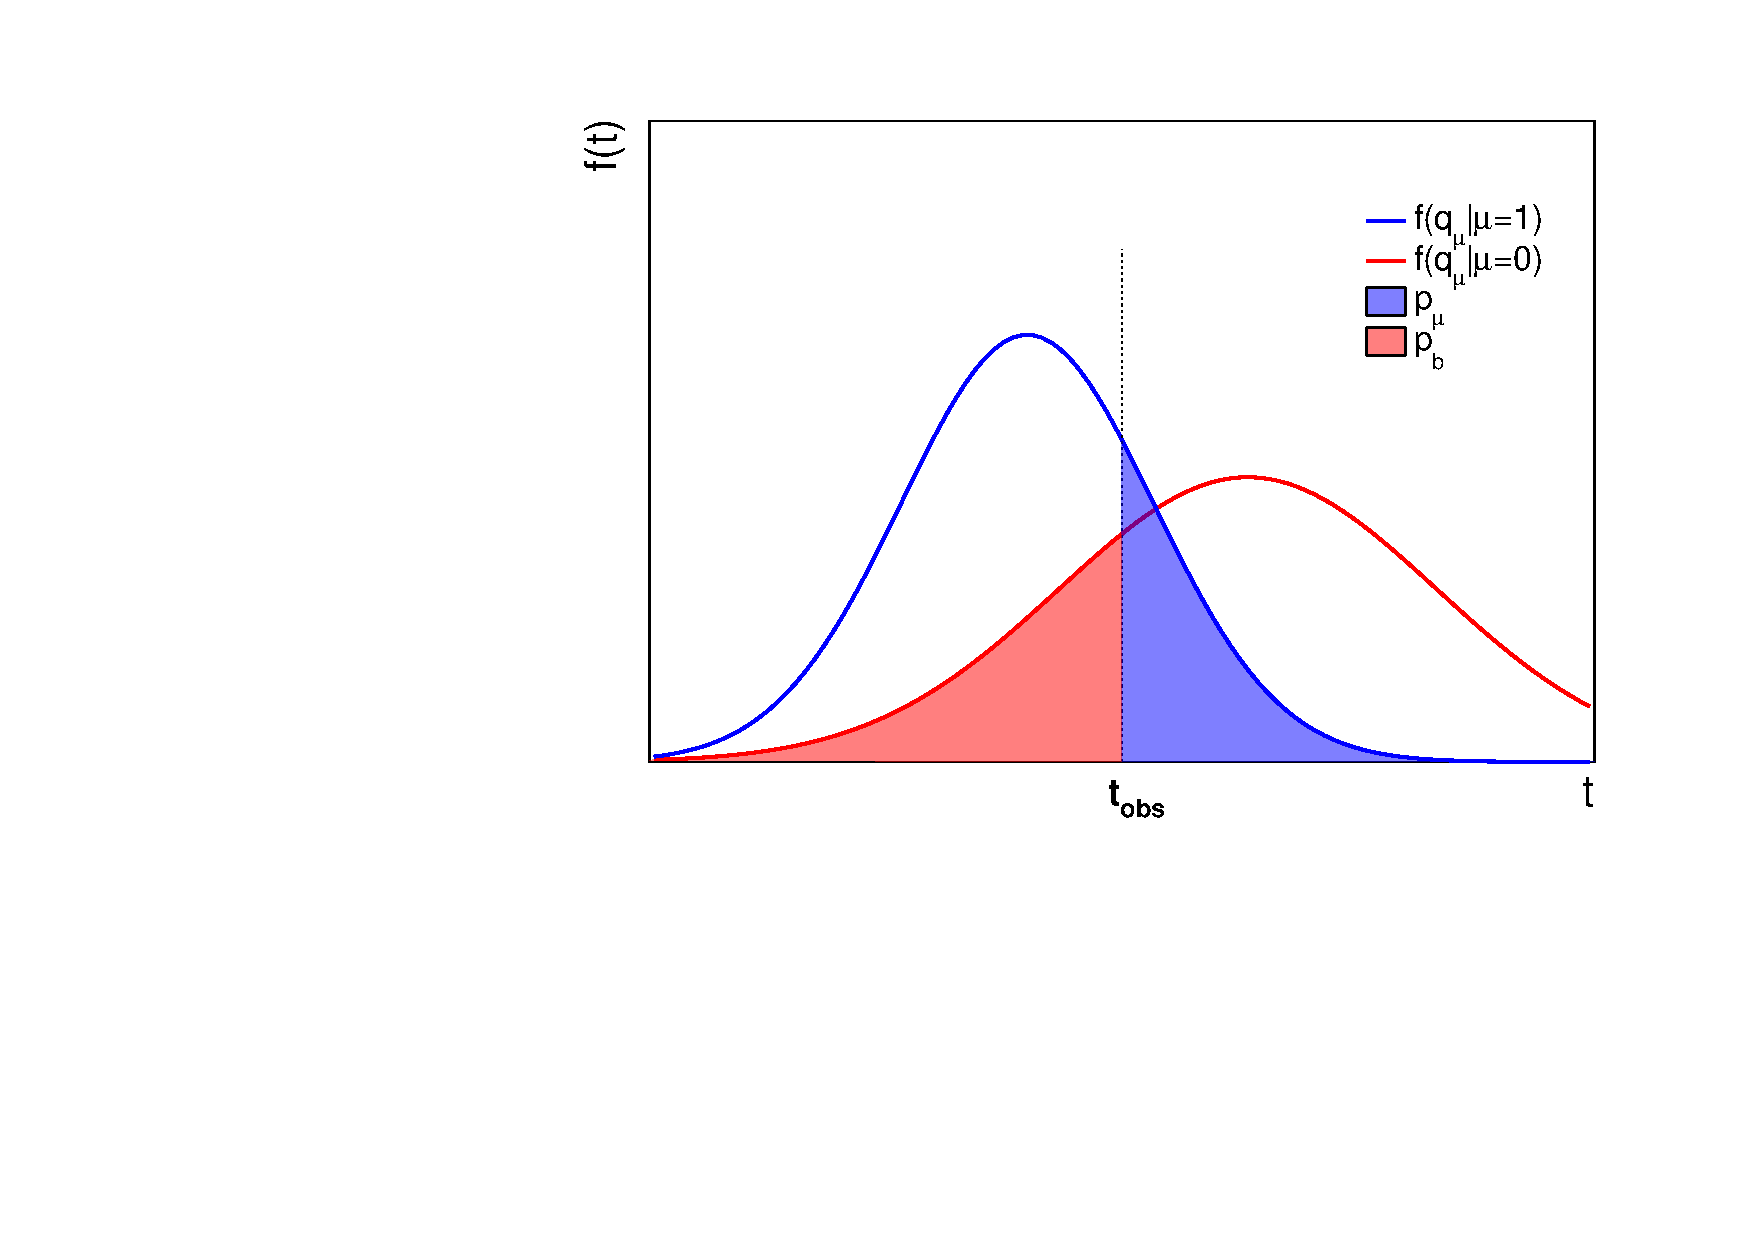
\includegraphics[width=0.8\textwidth]{produce_plots/stat/pmu_pb.pdf}
\caption{Distribution of the test statistic $q_\mu$ in the case of background only (red line) and signal-plus-background (blue line) hypothesis. The filled blue are indicates the value of $p_\mu$, while the filled red area indicated the value of $p_b$.}
\label{fig:stat:pmu_pb}
\end{figure}

\subsection{Distribution of the Test Statistic}

To compute the p-value associated with the observed value of a test statistics $t$, we need the PDF of $t$ assuming that the signal hypothesis $H_\mu$ is true, $ f(t | \mu ) $. The distribution of the test statistics can be obtained with pseudo-experiments or, in the case of large statistics, with the asymptotic approximation. 

\subsubsection*{Pseudo-experiments}

The distribution of the test statistic can be obtained by sampling the likelihood function with MC simulations (pseudo-experiments). This is obtained by repeating many times the following steps:
\begin{itemize}
\item The nominal value of all the nuisance parameters is varied randomly by sampling their constraining terms 
\item The new value of the nuisance parameters is used to compute a new expected value for the yields
\item The observed value is substituted by a Poisson fluctuation of the expected yields
\item The test statistic for this "observed" value is computed
\end{itemize}

This is done twice: a first time using as expected number of events the one predicted by the null hypothesis, and a second time the one predicted by the alternate hypothesis. The integral of the two resulting distributions is used to compute the p-values.

\subsubsection*{Asymptotic Approximation}
For large number of events, the asymptotic approximation \cite{Cowan2011} can be used to determine the \pdf of the test statistic without having to simulate a large number of pseudo-experiments. This technique is based on  Wald's theorem \cite{Wald1943}, which states that $t_{\mu} = -2 \ln \lambda(\mu)$ is parabolic up to corrections that scale with the inverse of the square root of the sample size:

\begin{equation}
\label{eq:wald}
t_{\mu} = -2 \ln \lambda(\mu)
= \frac{(\mu - \hat{\mu})^2}{\sigma^2} + {\cal  O}(1/\sqrt{N}) \;.
\end{equation}

\noindent Ignoring the ${\cal  O}(1/\sqrt{N})$ terms, $t_{\mu} = -2 \ln \lambda(\mu)$ is then distributed according to a noncentral chi-square distribution with one degree of freedom:

\begin{equation}
\label{eq:stat:ftmulambda}
f(t_{\mu};\Lambda) = \frac{1}{2 \sqrt{t_{\mu}}} \frac{1}{\sqrt{2 \pi}}
\left[ \exp \left( - \frac{1}{2}
\left( \sqrt{t_{\mu}} + \sqrt{\Lambda} \right)^2 \right) +
\exp \left( - \frac{1}{2} \left( \sqrt{t_{\mu}} - \sqrt{\Lambda} \right)^2
\right) \right] \;,
\end{equation}

\noindent where the noncentrality parameter $\Lambda$ is

\begin{equation}
\label{eq:stat:noncentrality}
\Lambda = \frac{(\mu - \mu^{\prime})^2}{\sigma^2} \;.
\end{equation}

The value of $\sigma$ can be estimated through the Asimov dataset, defined as the dataset that, when used to estimate the likelihood parameters, leads to their true values.

\section{Simplified Examples}

\subsection{CRs to Constrain Uncertainties}
\label{sec:example_cr}

\subsection{Improving the Sensitivity by Combining Regions}
\label{sec:example_combi}

